\documentclass[twoside]{article}


\usepackage[sc]{mathpazo} % Use the Palatino font
\usepackage[T1]{fontenc} % Use 8-bit encoding that has 256 glyphs
\linespread{1.3} % Line spacing - Palatino needs more space between lines
\usepackage{microtype} % Slightly tweak font spacing for aesthetics

\usepackage[hmarginratio=1:1,top=32mm,columnsep=20pt]{geometry} % Document margins
\usepackage{multicol} % Used for the two-column layout of the document
\usepackage[hang, small,labelfont=bf,up,textfont=it,up]{caption} % Custom captions under/above floats in tables or figures
\usepackage{booktabs} % Horizontal rules in tables
\usepackage{float} % Required for tables and figures in the multi-column environment - they need to be placed in specific locations with the [H] (e.g. \begin{table}[H])
\usepackage{hyperref} % For hyperlinks in the PDF

\usepackage{lettrine} % The lettrine is the first enlarged letter at the beginning of the text
\usepackage{paralist} % Used for the compactitem environment which makes bullet points with less space between them

\usepackage{titlesec} % Allows customization of titles
\renewcommand\thesection{\Roman{section}} % Roman numerals for the sections
\renewcommand\thesubsection{\Roman{subsection}} % Roman numerals for subsections
\titleformat{\section}[block]{\large\scshape\centering}{\thesection.}{1em}{} % Change the look of the section titles
\titleformat{\subsection}[block]{\large}{\thesubsection.}{1em}{} % Change the look of the section titles

\usepackage{fancyhdr} % Headers and footers
\pagestyle{fancy} % All pages have headers and footers
\fancyhead{} % Blank out the default header
\fancyfoot{} % Blank out the default footer
\fancyhead[C]{Melody Extraction} % Custom header text
\fancyfoot[RO,LE]{\thepage} % Custom footer text


\usepackage{multicol}
\usepackage{multirow}
% \setlength{\columnseprule}{0.4pt}
\usepackage{listings}
\usepackage{graphicx}
\usepackage{caption}
\usepackage{subcaption}
\usepackage{hyperref}
\usepackage{color}
\usepackage{float}
\usepackage{mathtools}
\usepackage{amssymb}
\usepackage{wrapfig}
\usepackage{amsmath}
\usepackage{xcolor}

\newcommand{\RN}[1]{%
  \textup{\uppercase\expandafter{\romannumeral#1}}%
}

% Default fixed font does not support bold face
\DeclareFixedFont{\ttb}{T1}{txtt}{bx}{n}{9} % for bold
\DeclareFixedFont{\ttm}{T1}{txtt}{m}{n}{9}  % for normal

% Custom colors
\usepackage{color}
\definecolor{deepblue}{rgb}{0,0,0.5}
\definecolor{deepred}{rgb}{0.6,0,0}
\definecolor{deepgreen}{rgb}{0,0.5,0}

\newcommand\pythonstyle{\lstset{
language=Python,
basicstyle=\ttm,
otherkeywords={self},             % Add keywords here
keywordstyle=\ttb\color{deepblue},
emph={MyClass,__init__},          % Custom highlighting
emphstyle=\ttb\color{deepred},    % Custom highlighting style
stringstyle=\color{deepgreen},
frame=tb,                         % Any extra options here
showstringspaces=false            % 
}}


% Python environment
\lstnewenvironment{python}[1][]
{
\pythonstyle
\lstset{#1}
}
{}

% Python for external files
\newcommand\pythonexternal[2][]{{
\pythonstyle
\lstinputlisting[#1]{#2}}}

% Python for inline
\newcommand\pythoninline[1]{{\pythonstyle\lstinline!#1!}}
%----------------------------------------------------------------------------------------
%	TITLE SECTION
%----------------------------------------------------------------------------------------

\title{\vspace{-15mm}\fontsize{24pt}{10pt}\selectfont\textbf{Summary of Melody Extraction}} % Article title

\author{
\large
\textsc{Li Yicheng}\thanks{\href{https://github.com/IAMLYCHEE?tab=repositories}{github link: https://github.com/IAMLYCHEE} }\\[2mm] % Your name
\normalsize t-yicli @ microsoft.com\\
\normalsize email: l.y.c.liyicheng@gmail.com \\ % Your institution
\normalsize Microsoft Xiao ICE \\
\vspace{-5mm}
}

\date{}
%----------------------------------------------------------------------------------------

\begin{document}
\section{Dependencies}
$\bullet$ Anaconda: Alternative , but recommended \\
$\bullet$ \href{https://github.com/librosa/librosa}{Librosa$\geq 0.6.1$}: \colorbox{gray!40}{pip install librosa}\\
$\bullet$ \href{http://www.scipy.org/}{NumPy $\geq 1.14.3$ \& SciPy$\geq 1.1.0$} \\
$\bullet$ \href{https://github.com/jiaaro/pydub}{pydub($\geq 0.22.0$)} \colorbox{gray!40}{pip install pydub}. \\
\textit{this is needed only when you would like to generate melody wav file with singletone audio.}\\
$\bullet$ \href{https://github.com/craffel/pretty-midi}{pretty-midi($\geq 0.2.8$)} \colorbox{gray!40}{pip install pretty\_midi}\\
\textit{this is needed only when you would like to generate melody midi file.}\\


\section{Application Mode}
\subsection{How to use}
1.Put your audio file into \textit{'wav'} folder\\
2.open your command line tool, (in Windows use cmd, in Linux use terminal) \\cd into folder where exist file \textit{'app.py'}\\
3.in command line tool, type : \colorbox{gray!40}{>python app.py filename [mode]}\\
\textit{\textbf{filename}: the audio filename you would like to process}\\
\textit{\textbf{mode}: three options , 'wav2wav' , 'wav2midi', or no input}\\

\subsection{Example}
if I have a file \textbf{'meiruoliming.wav'} in the \textbf{/wav} folder.
default mode:
\begin{figure}[H]
   \centering
   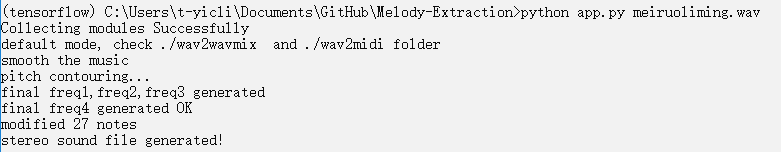
\includegraphics[width = 0.8\textwidth]{default.PNG}  
   \caption{no input in mode}
\end{figure}

wav2wav mode:
\begin{figure}[H]
   \centering
   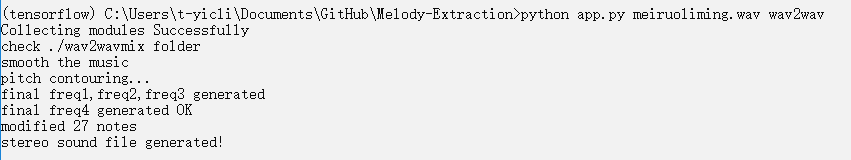
\includegraphics[width = 0.8\textwidth]{wav2wav.PNG}  
   \caption{wav2wav mode}
\end{figure}

wav2midi mode:
\begin{figure}[H]
   \centering
   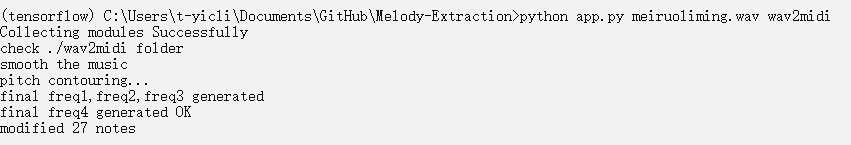
\includegraphics[width = 0.8\textwidth]{wav2midi.PNG}  
   \caption{wav2midi mode}
\end{figure}

\section{Developer mode}
some important functions you may need. 

\subsection{PitchInfo}
\subsubsection{audio\_notes, audio = PitchInfo.getNotesInfo()}
\textbf{audio\_notes}: a list of notes. each notes is in the form of start frame, end frame, estimated pitch.\\
\textbf{audio}: a numpy array showing the waveform data of the audio. \\

\noindent $\bullet$ \textbf{Example}
\begin{python}
from getPitchInfo import PitchInfo
pitch_info = PitchInfo('./wav/meiruoliming.wav')
notes,_ = pitch_info.getNotesInfo()
for note in notes:
	print(note)
#===========result============#
(47, 117, 57.82826990552989)
(117, 152, 57.650180126963406)
(152, 187, 59.89729843803559)
(187, 228, 59.89729843803559)
(256, 291, 60.66030413979112)
(291, 326, 61.391096674104446)
(326, 396, 62.76617800585667)
(396, 536, 62.09228621547197)
(536, 594, 62.281299902377036)
(686, 771, 59.89729843803559)
(834, 1044, 54.69532293693169)
(1044, 1079, 56.92606818447992)
........
#=============================#
\end{python}

\subsubsection{audio\_freq, audio = PitchInfo.getFreqInfo()}
\textbf{audio\_freq}: a numpy array aligned with the audio wave form data.\\
\textbf{audio}: a numpy array showing the waveform data of the audio \\





\end{document}